\documentclass[aspectratio=43,10pt]{beamer}

% Theme & Styling
\usetheme{Madrid}
\usecolortheme{whale}

% -----------------------------------------------------------------------------
% Elegant Obsidian / Dark Aesthetic Palette (Grant Sanderson 3Blue1Brown Style)
% -----------------------------------------------------------------------------
\definecolor{DarkCanvas}{RGB}{12, 16, 24}      % Deep obsidian canvas
\definecolor{DarkBox}{RGB}{20, 27, 40}         % Translucent dark card
\definecolor{DarkBoxInner}{RGB}{26, 36, 54}    % Accent box background
\definecolor{LuminousGold}{RGB}{245, 190, 60}  % Vibrant Gold / ITB Gold
\definecolor{ElectricBlue}{RGB}{80, 165, 250}  % Luminous Sky Blue
\definecolor{TealCyan}{RGB}{45, 212, 191}      % Cyan / Teal
\definecolor{EmeraldGreen}{RGB}{52, 211, 153}  % High-contrast green
\definecolor{CoralRose}{RGB}{251, 113, 133}    % High-contrast rose (Kendala/Peringatan)
\definecolor{PurpleBelok}{RGB}{216, 140, 255}  % Vivid lilac
\definecolor{SoftGray}{RGB}{200, 210, 225}     % Readable muted text

% Apply Dark Colors to Beamer Elements
\setbeamercolor{background canvas}{bg=DarkCanvas}
\setbeamercolor{normal text}{fg=white}
\setbeamercolor{structure}{fg=ElectricBlue}
\setbeamercolor{title}{fg=white,bg=DarkBox}
\setbeamercolor{frametitle}{fg=LuminousGold,bg=DarkBox}
\setbeamercolor{footline}{fg=SoftGray!70,bg=DarkCanvas}
\setbeamercolor{headline}{fg=SoftGray!70,bg=DarkCanvas}

% Block Styles in Dark Theme
\setbeamercolor{block title}{fg=white,bg=ElectricBlue!45!black}
\setbeamercolor{block body}{fg=white,bg=DarkBox}
\setbeamercolor{block title example}{fg=white,bg=EmeraldGreen!40!black}
\setbeamercolor{block body example}{fg=white,bg=DarkBox}
\setbeamercolor{block title alerted}{fg=white,bg=CoralRose!45!black}
\setbeamercolor{block body alerted}{fg=white,bg=DarkBox}

% Lists & Numbering
\setbeamercolor{item}{fg=LuminousGold}
\setbeamercolor{subitem}{fg=TealCyan}
\setbeamercolor{enumerate item}{fg=LuminousGold}
\setbeamercolor{enumerate subitem}{fg=TealCyan}

% Packages
\usepackage[utf8]{inputenc}
\usepackage{amsmath,amssymb}
\usepackage{graphicx}
\usepackage{hyperref}
\usepackage{multimedia}
\usepackage{tikz}

\hypersetup{
    colorlinks=true,
    linkcolor=TealCyan,
    urlcolor=ElectricBlue
}

\title[MA1101 Matematika I]{MA1101 Matematika I --- Bab 5: Penggunaan Integral}
\subtitle{Subtopik 5.3: Volume Benda Putar: Metode Kulit Tabung\\(\textit{Volumes of Solids: Cylindrical Shells})}
\author[FMIPA ITB]{Tim Pengajar MA1101}
\institute[ITB]{Fakultas Matematika dan Ilmu Pengetahuan Alam\\Institut Teknologi Bandung}
\date{Semester 1 Tahun Akademik 2026/2027}

\begin{document}

% -------------------------------------------------------------
% Slide 1: Judul
% -------------------------------------------------------------
\begin{frame}
    \titlepage
\end{frame}

% -------------------------------------------------------------
% Slide 2: Motivasi Metode Kulit Tabung
% -------------------------------------------------------------
\begin{frame}{Motivasi: Mengapa Metode Cakram \& Cincin Tidak Selalu Cukup?}
    \begin{block}{Dilema Memutar $y = f(x)$ Mengelilingi Sumbu-$y$}
        \scriptsize
        Pada Subtopik 5.2.a, memutar daerah mengelilingi \textbf{sumbu-$y$} dengan Metode Cakram/Cincin mengharuskan kita mengambil \textbf{pias mendatar ($\Delta y \perp$ sumbu-$y$)} dan menyatakan $x$ sebagai fungsi dari $y$. Namun, perhatikan dua masalah klasik berikut:
    \end{block}

    \begin{columns}[T]
        \begin{column}{0.48\textwidth}
            \begin{alertblock}{1. Kurva Sulit / Mustahil Diinvers}
                \scriptsize
                Misalkan daerah di bawah kurva kubik:
                $$y = 2x^2 - x^3 \quad\text{pada } [0, 2]$$
                diputar mengelilingi \textbf{sumbu-$y$}.\\
                \vskip 2pt
                Dengan pias mendatar ($\Delta y$), baik ujung kanan maupun ujung kiri pias menempel pada kurva yang sama! Menyelesaikan $x^3 - 2x^2 + y = 0$ untuk $x = g(y)$ sangat rumit.
            \end{alertblock}
        \end{column}

        \begin{column}{0.48\textwidth}
            \begin{exampleblock}{2. Integral Menjadi Jauh Lebih Mudah}
                \scriptsize
                Misalkan daerah di bawah:
                $$y = \sin(x^2) \quad\text{pada } \big[0, \sqrt{\pi}\big]$$
                diputar mengelilingi \textbf{sumbu-$y$}.\\
                \vskip 2pt
                Dengan Metode Kulit Tabung ($\Delta x \parallel$ sumbu-$y$), kita akan memperoleh faktor $\mathbf{x}$ di depan $\sin(x^2)$, sehingga $\int 2\pi x\sin(x^2)\,dx$ langsung selesai dengan substitusi $u = x^2$!
            \end{exampleblock}
        \end{column}
    \end{columns}
\end{frame}

% -------------------------------------------------------------
% Slide 3: Geometri Satu Kulit Tabung (Iris dan Bentangkan)
% -------------------------------------------------------------
\begin{frame}{Geometri Satu Kulit Tabung (\textit{Cylindrical Shell})}
    \begin{columns}[c]
        \begin{column}{0.54\textwidth}
            \begin{block}{Penurunan Aljabar \& Tafsiran ``Iris dan Bentangkan''}
                \scriptsize\abovedisplayskip=2pt\belowdisplayskip=2pt
                Sebuah kulit tabung (silinder berongga berdinding tipis) dengan jari-jari dalam $r_1$, jari-jari luar $r_2$, jari-jari rata-rata $\mathbf{r = \frac{1}{2}(r_1 + r_2)}$, tinggi $\mathbf{h}$, dan tebal $\mathbf{\Delta r = r_2 - r_1}$ memiliki volume eksak:
                \begin{align*}
                    \Delta V &= \pi r_2^2 h - \pi r_1^2 h = \pi(r_2 + r_1)(r_2 - r_1)h\\
                    &= 2\pi\!\left(\frac{r_2 + r_1}{2}\right)\!h\,\Delta r = \mathbf{2\pi r h\,\Delta r}.
                \end{align*}
                Jika kulit tabung dibelah vertikal dan \textbf{dibentangkan rata menjadi balok}:
            \end{block}
            {\scriptsize$$\boxed{\;\Delta V \approx (\text{keliling})\cdot(\text{tinggi})\cdot(\text{tebal}) = 2\pi r \cdot h \cdot \Delta r\;}$$}
        \end{column}

        \begin{column}{0.43\textwidth}
            \centering
            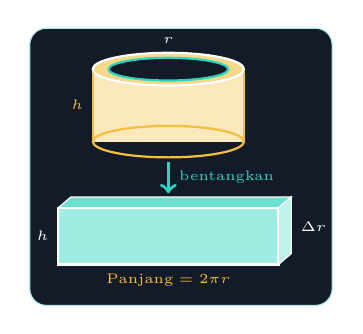
\begin{tikzpicture}[scale=0.8]
                \draw[fill=DarkBox, draw=TealCyan!40, rounded corners=6pt] (-2.2,-2.1) rectangle (2.6,2.3);
                % Kulit tabung di atas
                \fill[color=LuminousGold!35] (-1.2,0.5) rectangle (1.2,1.65);
                \draw[color=LuminousGold, thick] (-1.2,0.5) -- (-1.2,1.65);
                \draw[color=LuminousGold, thick] (1.2,0.5) -- (1.2,1.65);
                \draw[color=LuminousGold, thick] (0,0.5) ellipse (1.2 and 0.25);
                \fill[color=LuminousGold!60, draw=white, thick] (0,1.65) ellipse (1.2 and 0.26);
                \fill[color=DarkBox, draw=TealCyan, thick] (0,1.65) ellipse (0.95 and 0.18);
                \node[left, color=LuminousGold] at (-1.2,1.08) {\tiny $h$};
                \node[above, color=white] at (0,1.9) {\tiny $r$};
                % Panah bentangkan ke balok di bawah
                \draw[->, color=TealCyan, line width=1.2pt] (0,0.18) -- (0,-0.32) node[midway, right] {\tiny bentangkan};
                % Balok rata di bawah
                \fill[color=TealCyan!45, draw=white, thick] (-1.75,-1.45) rectangle (1.75,-0.55);
                \fill[color=TealCyan!70, draw=white] (-1.75,-0.55) -- (1.75,-0.55) -- (1.95,-0.38) -- (-1.55,-0.38) -- cycle;
                \fill[color=TealCyan!30, draw=white] (1.75,-1.45) -- (1.95,-1.28) -- (1.95,-0.38) -- (1.75,-0.55) -- cycle;
                \node[below, color=LuminousGold] at (0,-1.45) {\tiny $\text{Panjang} = 2\pi r$};
                \node[left, color=white] at (-1.75,-1.0) {\tiny $h$};
                \node[right, color=white] at (1.95,-0.85) {\tiny $\Delta r$};
            \end{tikzpicture}
        \end{column}
    \end{columns}
\end{frame}

% -------------------------------------------------------------
% Slide 4: Rumus Metode Kulit Tabung Mengelilingi Sumbu-y
% -------------------------------------------------------------
\begin{frame}{Metode Kulit Tabung Mengelilingi Sumbu-$y$ ($\Delta x \parallel$ Sumbu-$y$)}
    \begin{block}{Teorema / Rumus Metode Kulit Tabung (Putar Sumbu-$y$)}
        \scriptsize\abovedisplayskip=3pt\belowdisplayskip=3pt
        Misalkan daerah dibatasi oleh kurva $y = f(x) \ge 0$, sumbu-$x$, serta garis $x = a$ dan $x = b$ (dengan $0 \le a < b$). Jika daerah tersebut diputar $360^\circ$ mengelilingi \textbf{sumbu-$y$}, maka pias tegak pada posisi $x$ (selebar $\Delta x \parallel$ sumbu-$y$) menyapu kulit tabung dengan \textbf{jari-jari $r(x) = x$} dan \textbf{tinggi $h(x) = f(x)$}:
        $$\boxed{\;\Delta V \approx 2\pi x\,f(x)\,\Delta x \implies V = 2\pi\int_{a}^{b} \underbrace{x}_{\text{jari-jari}}\cdot\underbrace{f(x)}_{\text{tinggi}}\,dx\;}$$
    \end{block}

    \begin{columns}[T]
        \begin{column}{0.48\textwidth}
            \begin{exampleblock}{Ciri Khas Metode Kulit Tabung}
                \scriptsize
                \begin{itemize}\itemsep=2pt
                    \item Pias diambil \textbf{SEJAJAR ($\parallel$) dengan sumbu putar} (\textit{bukan} tegak lurus!).
                    \item Pengali di depan integral adalah $\mathbf{2\pi}$ (berasal dari keliling lingkaran $2\pi r$, bukan luas $\pi R^2$).
                \end{itemize}
            \end{exampleblock}
        \end{column}

        \begin{column}{0.48\textwidth}
            \begin{alertblock}{Jari-Jari Berpangkat Satu!}
                \scriptsize
                \begin{itemize}\itemsep=2pt
                    \item Pada Metode Cakram/Cincin: jari-jari dikuadratkan ($\pi R^2$).
                    \item Pada Metode Kulit Tabung: jari-jari $r = x$ \textbf{dikalikan dengan tinggi $h = f(x)$} ($2\pi x f(x)$).
                \end{itemize}
            \end{alertblock}
        \end{column}
    \end{columns}
\end{frame}

% -------------------------------------------------------------
% Slide 5: Simulasi Video 1 - CylindricalShellsUnrollingScene
% -------------------------------------------------------------
\begin{frame}{Simulasi Dinamis: Kulit Tabung \& Pembentangan Balok ($2\pi x\,f(x)\,\Delta x$)}
    \centering
    \movie[width=0.66\textwidth,height=0.44\textwidth,poster,showcontrols=true]%
        {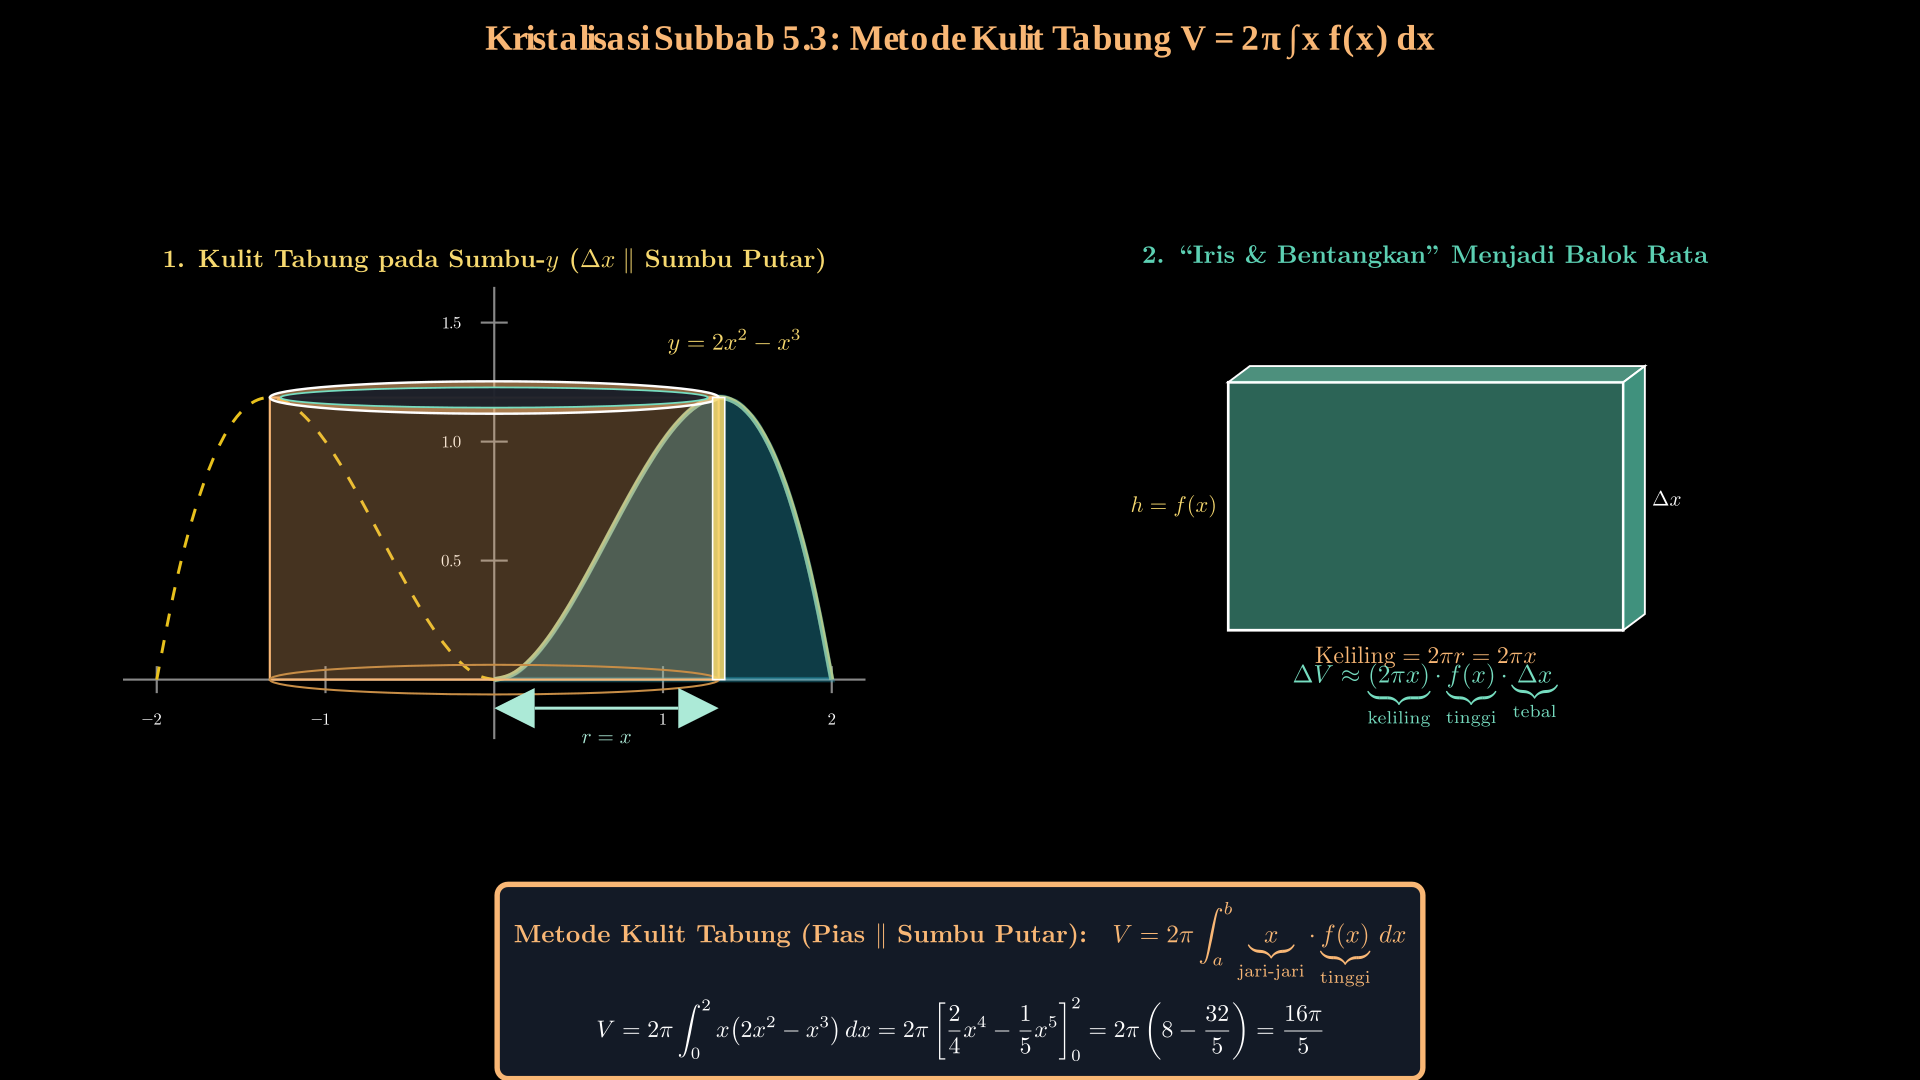
\includegraphics[width=0.66\textwidth,height=0.44\textwidth]{keyframe_kulit_tabung_bentang.png}}%
        {CylindricalShellsUnrollingScene.ogv}

    \vskip 0.2em
    \href{run:./play_video.sh bentang}{%
        \beamerbutton{\small\color{white} $\blacktriangleright$ Putar Video Animasi (\texttt{CylindricalShellsUnrollingScene.mp4})}%
    }

    \vskip 0.2em
    \tiny\textit{\color{SoftGray}Perhatikan bagaimana pias tegak ($\Delta x \parallel$ sumbu-$y$) menyapu kulit tabung dan dibentangkan menjadi balok $2\pi x\cdot f(x)\cdot\Delta x$.}
\end{frame}

% -------------------------------------------------------------
% Slide 6: Contoh 1 - Menyelesaikan Masalah Pembuka (Kubik & Substitusi)
% -------------------------------------------------------------
\begin{frame}{Contoh 1: Menyelesaikan Masalah Pembuka dengan Kulit Tabung}
    \begin{columns}[T]
        \begin{column}{0.48\textwidth}
            \begin{exampleblock}{Soal 1A: Kurva Kubik $y = 2x^2 - x^3$}
                \scriptsize\abovedisplayskip=2pt\belowdisplayskip=2pt
                Daerah $R$ dibatasi oleh $y = 2x^2 - x^3$ dan sumbu-$x$ pada $[0, 2]$. Hitunglah volume benda yang terbentuk jika $R$ diputar mengelilingi \textbf{sumbu-$y$}!
                \vskip 3pt
                \textbf{Penyelesaian}:\\
                Ambil pias tegak ($\Delta x \parallel$ sumbu-$y$). Pada posisi $x \in [0, 2]$, jari-jari kulit tabung $r = x$ dan tingginya $h = 2x^2 - x^3$:
                \begin{align*}
                    V &= 2\pi\int_{0}^{2} x\big(2x^2 - x^3\big)\,dx\\
                    &= 2\pi\int_{0}^{2} \big(2x^3 - x^4\big)\,dx\\
                    &= 2\pi\left[\frac{1}{2}x^4 - \frac{1}{5}x^5\right]_{0}^{2} = 2\pi\!\left(8 - \frac{32}{5}\right) = \mathbf{\frac{16\pi}{5}}.
                \end{align*}
            \end{exampleblock}
        \end{column}

        \begin{column}{0.48\textwidth}
            \begin{block}{Soal 1B: Kurva $y = \sin(x^2)$ pada $[0, \sqrt{\pi}]$}
                \scriptsize\abovedisplayskip=2pt\belowdisplayskip=2pt
                Daerah di bawah $y = \sin(x^2)$ pada $\big[0, \sqrt{\pi}\big]$ diputar mengelilingi \textbf{sumbu-$y$}. Tentukan volumenya!
                \vskip 3pt
                \textbf{Penyelesaian}:\\
                Dengan Metode Kulit Tabung ($\Delta x \parallel$ sumbu-$y$):
                $$V = 2\pi\int_{0}^{\sqrt{\pi}} x\sin(x^2)\,dx.$$
                Substitusi $u = x^2 \implies du = 2x\,dx$ (batas $u = 0$ sampai $u = \pi$):
                $$V = \pi\int_{0}^{\pi} \sin u\,du = \pi\big[-\cos u\big]_{0}^{\pi} = \mathbf{2\pi}.$$
                {\tiny\color{TealCyan}Faktor $x$ dari jari-jari kulit tabung justru menyelamatkan integral!}
            \end{block}
        \end{column}
    \end{columns}
\end{frame}

% -------------------------------------------------------------
% Slide 7: Contoh 2 - Membandingkan Cincin vs Kulit Tabung pada Benda yang Sama
% -------------------------------------------------------------
\begin{frame}{Contoh 2: Metode Cincin vs.\ Kulit Tabung pada Benda yang Sama}
    \begin{exampleblock}{Soal (Purcell \S5.3)}
        \scriptsize
        Daerah $R$ dibatasi oleh $y = \sqrt{x}$, sumbu-$x$ ($y = 0$), dan garis $x = 4$. Hitung volume benda putar jika $R$ diputar mengelilingi \textbf{sumbu-$y$} menggunakan \textbf{(a) Metode Cincin} dan \textbf{(b) Metode Kulit Tabung}!
    \end{exampleblock}

    \begin{columns}[T]
        \begin{column}{0.48\textwidth}
            \begin{block}{(a) Metode Cincin (Pias Mendatar $\Delta y \perp$ Sumbu-$y$)}
                \scriptsize\abovedisplayskip=2pt\belowdisplayskip=2pt
                Untuk $y \in [0, 2]$, batas kanan adalah garis $x = 4$ dan batas kiri adalah parabola $x = y^2$:
                $$R_{\text{luar}}(y) = 4, \qquad r_{\text{dalam}}(y) = y^2.$$
                Maka:
                \begin{align*}
                    V &= \pi\int_{0}^{2} \Big[4^2 - (y^2)^2\Big]\,dy\\
                    &= \pi\left[16y - \frac{y^5}{5}\right]_{0}^{2} = \pi\!\left(32 - \frac{32}{5}\right) = \mathbf{\frac{128\pi}{5}}.
                \end{align*}
            \end{block}
        \end{column}

        \begin{column}{0.48\textwidth}
            \begin{alertblock}{(b) Metode Kulit Tabung (Pias Tegak $\Delta x \parallel$ Sumbu-$y$)}
                \scriptsize\abovedisplayskip=2pt\belowdisplayskip=2pt
                Untuk $x \in [0, 4]$, pias tegak memiliki jari-jari $r(x) = x$ dan tinggi $h(x) = \sqrt{x}$:
                $$\Delta V \approx 2\pi x\sqrt{x}\,\Delta x = 2\pi x^{3/2}\,\Delta x.$$
                Maka:
                \begin{align*}
                    V &= 2\pi\int_{0}^{4} x^{3/2}\,dx\\
                    &= 2\pi\left[\frac{2}{5}x^{5/2}\right]_{0}^{4} = \frac{4\pi}{5}(32) = \mathbf{\frac{128\pi}{5}}.
                \end{align*}
            \end{alertblock}
        \end{column}
    \end{columns}
\end{frame}

% -------------------------------------------------------------
% Slide 8: Kulit Tabung di Antara Dua Kurva
% -------------------------------------------------------------
\begin{frame}{Metode Kulit Tabung untuk Daerah di Antara Dua Kurva}
    \begin{block}{Rumus Kulit Tabung di Antara $y = f(x)$ dan $y = g(x)$ (Putar Sumbu-$y$)}
        \scriptsize\abovedisplayskip=2pt\belowdisplayskip=2pt
        Jika daerah dibatasi oleh kurva atas $y = f(x)$ dan kurva bawah $y = g(x)$ pada $[a, b]$ ($0 \le a < b$ dan $f(x) \ge g(x)$), maka tinggi pias tegak pada posisi $x$ adalah $\mathbf{h(x) = f(x) - g(x)}$, sehingga:
        $$\boxed{\;\Delta V \approx 2\pi x\,\big[f(x) - g(x)\big]\,\Delta x \implies V = 2\pi\int_{a}^{b} x\,\big[f(x) - g(x)\big]\,dx\;}$$
    \end{block}

    \begin{exampleblock}{Contoh 3: Daerah di Antara Dua Parabola Diputar Mengelilingi Sumbu-$y$}
        \scriptsize\abovedisplayskip=2pt\belowdisplayskip=2pt
        Tentukan volume benda yang terbentuk jika daerah yang dibatasi oleh $y = 2x - x^2$ dan $y = x^2$ diputar mengelilingi \textbf{sumbu-$y$}!
        \begin{itemize}\itemsep=1pt
            \item Titik potong: $2x - x^2 = x^2 \iff 2x(1 - x) = 0 \implies \mathbf{x = 0}$ dan $\mathbf{x = 1}$.
            \item Pada $[0, 1]$, kurva atas adalah $y = 2x - x^2$ dan kurva bawah adalah $y = x^2$, sehingga tinggi kulit tabung adalah $h(x) = (2x - x^2) - x^2 = 2x - 2x^2$:
            $$V = 2\pi\int_{0}^{1} x\big(2x - 2x^2\big)\,dx = 4\pi\int_{0}^{1} \big(x^2 - x^3\big)\,dx = 4\pi\left[\frac{x^3}{3} - \frac{x^4}{4}\right]_{0}^{1} = \mathbf{\frac{\pi}{3}}.$$
        \end{itemize}
    \end{exampleblock}
\end{frame}

% -------------------------------------------------------------
% Slide 9: Metode Kulit Tabung Mengelilingi Sumbu-x (Pias Mendatar Δy)
% -------------------------------------------------------------
\begin{frame}{Metode Kulit Tabung Mengelilingi Sumbu-$x$ (Pias Mendatar $\Delta y$)}
    \begin{block}{Pias Mendatar ($\Delta y \parallel$ Sumbu-$x$) Diputar Mengelilingi Sumbu-$x$}
        \scriptsize\abovedisplayskip=2pt\belowdisplayskip=2pt
        Jika daerah dibatasi oleh kurva kanan $x = p(y)$ dan kurva kiri $x = q(y)$ untuk $y \in [c, d]$ ($c \ge 0$) lalu diputar mengelilingi \textbf{sumbu-$x$}, maka \textbf{pias mendatar ($\Delta y \parallel$ sumbu-$x$)} menyapu kulit tabung berjari-jari $\mathbf{r(y) = y}$ dan panjang $\mathbf{h(y) = p(y) - q(y)}$:
        $$\boxed{\;\Delta V \approx 2\pi y\,\big[p(y) - q(y)\big]\,\Delta y \implies V = 2\pi\int_{c}^{d} y\,\big(x_{\text{kanan}} - x_{\text{kiri}}\big)\,dy\;}$$
    \end{block}

    \begin{exampleblock}{Contoh 4: Mengapa Pias Mendatar ($\Delta y$) Menghemat Waktu?}
        \scriptsize\abovedisplayskip=2pt\belowdisplayskip=2pt
        Daerah di kuadran pertama yang dibatasi oleh parabola $x = y^2$, sumbu-$x$ ($y = 0$), dan garis $x + y = 2$ diputar mengelilingi \textbf{sumbu-$x$}. Hitunglah volumenya!
        \begin{itemize}\itemsep=1pt
            \item Jika memakai Metode Cakram ($\Delta x \perp$ sumbu-$x$), batas atas berganti di $x = 1$ (harus pecah 2 integral!).
            \item Sebaliknya, dengan \textbf{Metode Kulit Tabung ($\Delta y \parallel$ sumbu-$x$)} untuk $y \in [0, 1]$, batas kanan selalu garis $x_{\text{kanan}} = 2 - y$ dan batas kiri selalu parabola $x_{\text{kiri}} = y^2$:
            $$V = 2\pi\int_{0}^{1} y\big(2 - y - y^2\big)\,dy = 2\pi\left[y^2 - \frac{y^3}{3} - \frac{y^4}{4}\right]_{0}^{1} = 2\pi\left(\frac{5}{12}\right) = \mathbf{\frac{5\pi}{6}}.$$
        \end{itemize}
    \end{exampleblock}
\end{frame}

% -------------------------------------------------------------
% Slide 10: Rotasi Mengelilingi Garis Sejajar Sumbu Koordinat (x = k atau y = k)
% -------------------------------------------------------------
\begin{frame}{Kulit Tabung Mengelilingi Garis $x = k$ atau $y = k$}
    \begin{block}{Aturan Pengukuran Jari-Jari Kulit Tabung Terhadap Sumbu Putar Bergeser}
        \scriptsize
        Jika daerah diputar mengelilingi garis tegak $x = k$ atau garis mendatar $y = k$ yang berada di luar daerah, \textbf{tinggi kulit tabung $h$ TIDAK BERUBAH}, tetapi \textbf{jari-jari $r$ adalah jarak dari pias ke garis sumbu putar}:
    \end{block}

    \begin{columns}[T]
        \begin{column}{0.48\textwidth}
            \begin{exampleblock}{1. Putar Garis Tegak $x = k$ (Pias Tegak $\Delta x$)}
                \scriptsize\abovedisplayskip=2pt\belowdisplayskip=2pt
                Jari-jari kulit tabung pada posisi $x \in [a, b]$ adalah $r(x) = |x - k|$:
                \begin{itemize}\itemsep=2pt
                    \item Jika sumbu $x = k$ di \textbf{kiri} daerah ($x \ge k$):
                    $$\mathbf{r(x) = x - k}.$$
                    \item Jika sumbu $x = k$ di \textbf{kanan} daerah ($x \le k$):
                    $$\mathbf{r(x) = k - x}.$$
                \end{itemize}
                $$V = 2\pi\int_{a}^{b} |x - k|\cdot\big[f(x) - g(x)\big]\,dx.$$
            \end{exampleblock}
        \end{column}

        \begin{column}{0.48\textwidth}
            \begin{alertblock}{2. Putar Garis Mendatar $y = k$ (Pias Mendatar $\Delta y$)}
                \scriptsize\abovedisplayskip=2pt\belowdisplayskip=2pt
                Jari-jari kulit tabung pada ketinggian $y \in [c, d]$ adalah $r(y) = |y - k|$:
                \begin{itemize}\itemsep=2pt
                    \item Jika sumbu $y = k$ di \textbf{bawah} daerah ($y \ge k$):
                    $$\mathbf{r(y) = y - k}.$$
                    \item Jika sumbu $y = k$ di \textbf{atas} daerah ($y \le k$):
                    $$\mathbf{r(y) = k - y}.$$
                \end{itemize}
                $$V = 2\pi\int_{c}^{d} |y - k|\cdot\big[p(y) - q(y)\big]\,dy.$$
            \end{alertblock}
        \end{column}
    \end{columns}
\end{frame}

% -------------------------------------------------------------
% Slide 11: Simulasi Video 2 - ShellsVsWashersShiftedAxisScene
% -------------------------------------------------------------
\begin{frame}{Simulasi Dinamis: Kulit Tabung Terhadap Sumbu-$y$ vs.\ Garis $x = 2$}
    \centering
    \movie[width=0.66\textwidth,height=0.44\textwidth,poster,showcontrols=true]%
        {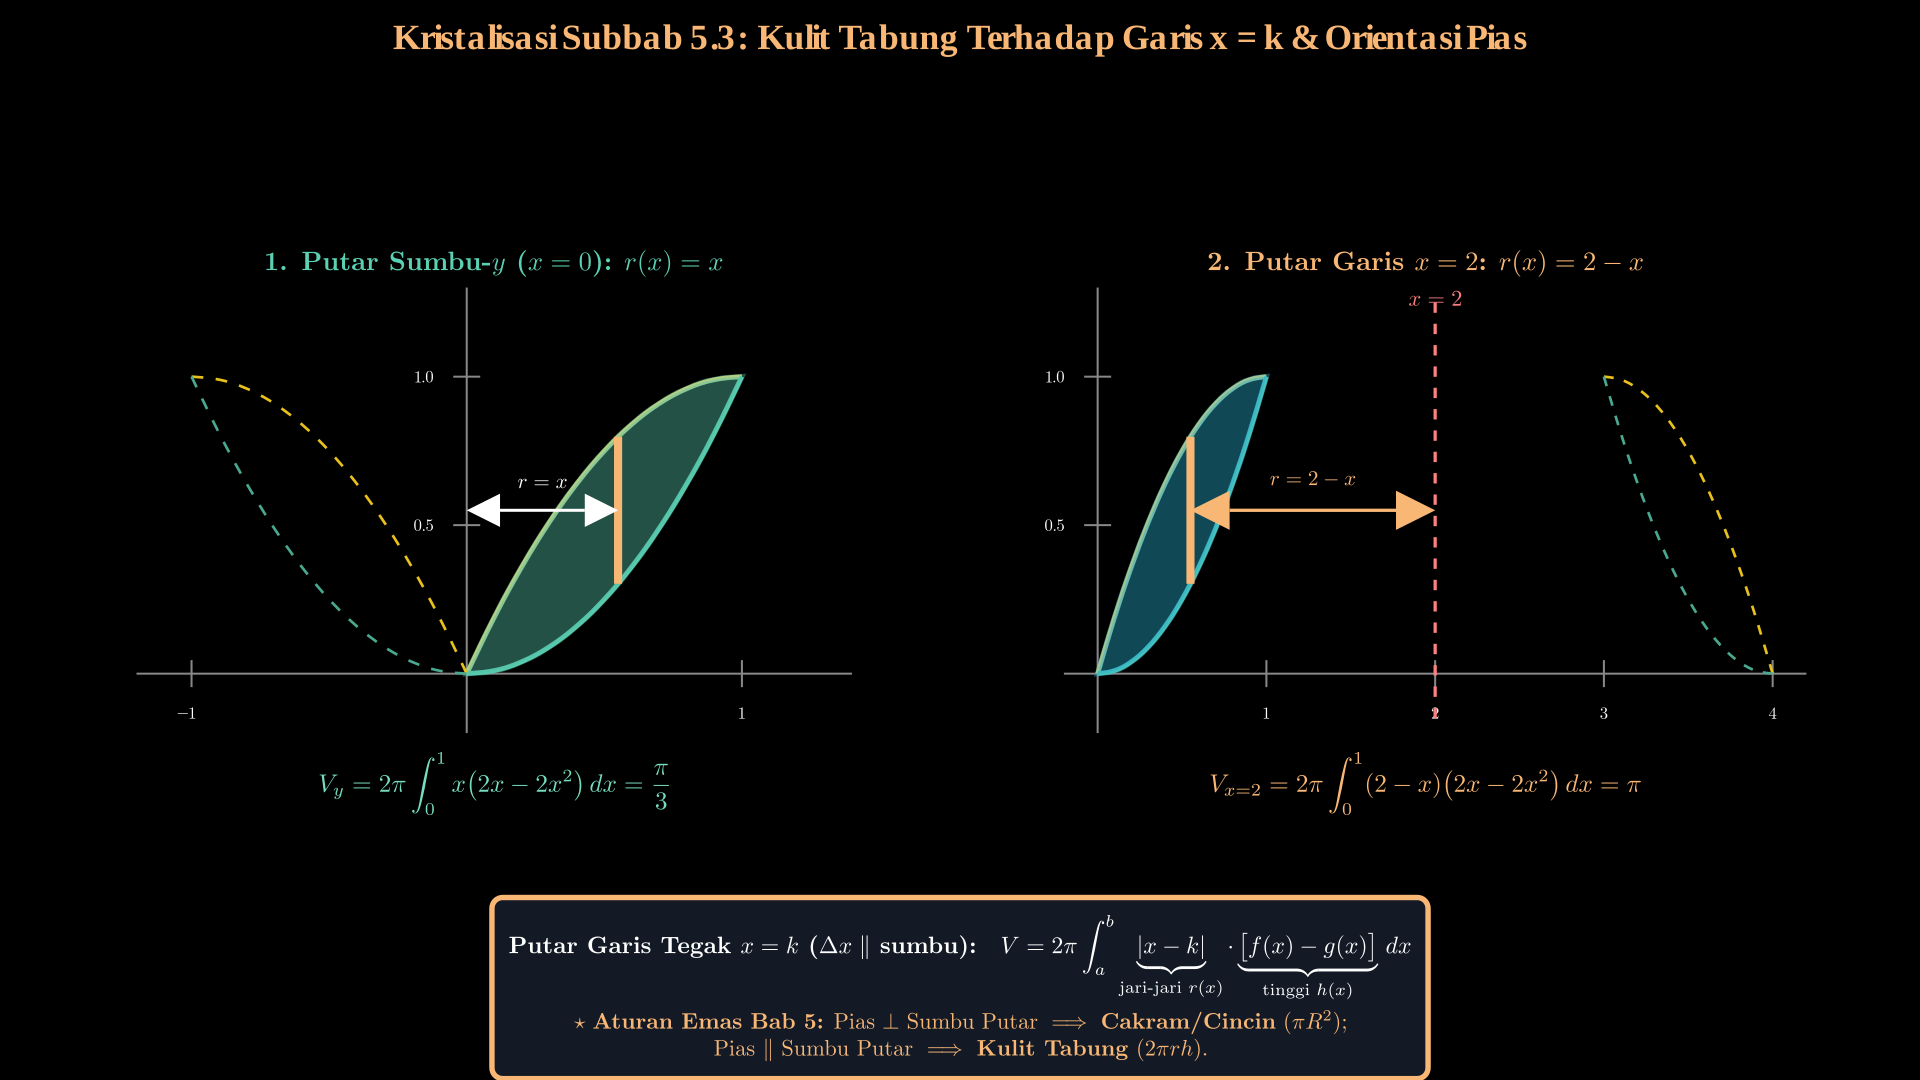
\includegraphics[width=0.66\textwidth,height=0.44\textwidth]{keyframe_kulit_tabung_geser.png}}%
        {ShellsVsWashersShiftedAxisScene.ogv}

    \vskip 0.2em
    \href{run:./play_video.sh geser}{%
        \beamerbutton{\small\color{white} $\blacktriangleright$ Putar Video Animasi (\texttt{ShellsVsWashersShiftedAxisScene.mp4})}%
    }

    \vskip 0.2em
    \tiny\textit{\color{SoftGray}Bandingkan bagaimana jari-jari kulit tabung berubah dari $r(x) = x$ (terhadap sumbu-$y$) menjadi $r(x) = 2 - x$ (terhadap garis $x = 2$).}
\end{frame}

% -------------------------------------------------------------
% Slide 12: Contoh 5 - Rotasi Terhadap Garis di Kanan (x = 2) vs di Kiri (x = -1)
% -------------------------------------------------------------
\begin{frame}{Contoh 5: Rotasi Mengelilingi Garis $x = 2$ vs.\ Garis $x = -1$}
    \begin{exampleblock}{Soal}
        \scriptsize
        Daerah $R$ dibatasi oleh $y = 2x - x^2$ dan $y = x^2$ pada $[0, 1]$ (tinggi pias tegak $h(x) = 2x - 2x^2$). Hitung volume benda putar jika $R$ diputar mengelilingi \textbf{(a) garis $x = 2$} dan \textbf{(b) garis $x = -1$}!
    \end{exampleblock}

    \begin{columns}[T]
        \begin{column}{0.48\textwidth}
            \begin{block}{(a) Mengelilingi Garis $x = 2$ (di Kanan $R$)}
                \scriptsize\abovedisplayskip=2pt\belowdisplayskip=2pt
                Karena $x \in [0, 1]$ berada di sebelah \textbf{kiri} garis $x = 2$, jarak pias ke sumbu putar adalah $\mathbf{r(x) = 2 - x}$:
                \begin{align*}
                    V &= 2\pi\int_{0}^{1} (2 - x)(2x - 2x^2)\,dx\\
                    &= 4\pi\int_{0}^{1} \big(2x - 3x^2 + x^3\big)\,dx\\
                    &= 4\pi\left[x^2 - x^3 + \frac{x^4}{4}\right]_{0}^{1} = \mathbf{\pi}.
                \end{align*}
            \end{block}
        \end{column}

        \begin{column}{0.48\textwidth}
            \begin{alertblock}{(b) Mengelilingi Garis $x = -1$ (di Kiri $R$)}
                \scriptsize\abovedisplayskip=2pt\belowdisplayskip=2pt
                Karena $x \in [0, 1]$ berada di sebelah \textbf{kanan} garis $x = -1$, jarak pias ke sumbu putar adalah $\mathbf{r(x) = x - (-1) = x + 1}$:
                \begin{align*}
                    V &= 2\pi\int_{0}^{1} (x + 1)(2x - 2x^2)\,dx\\
                    &= 4\pi\int_{0}^{1} \big(x - x^3\big)\,dx\\
                    &= 4\pi\left[\frac{x^2}{2} - \frac{x^4}{4}\right]_{0}^{1} = \mathbf{\pi}.
                \end{align*}
            \end{alertblock}
        \end{column}
    \end{columns}
\end{frame}

% -------------------------------------------------------------
% Slide 13: Contoh 6 - Rotasi Mengelilingi Garis Mendatar y = k dengan Pias Mendatar (Δy)
% -------------------------------------------------------------
\begin{frame}{Contoh 6: Kulit Tabung Mengelilingi Garis Mendatar $y = -1$ dan $y = 4$}
    \begin{exampleblock}{Soal}
        \scriptsize
        Daerah $R$ dibatasi oleh parabola $x = y^2$ dan garis $x = y + 2$ (berpotongan di $y = -1$ dan $y = 2$). Gunakan \textbf{Metode Kulit Tabung ($\Delta y$)} untuk menyusun dan menghitung volume jika $R$ diputar mengelilingi \textbf{(a) garis $y = -1$} dan \textbf{(b) garis $y = 3$}!
    \end{exampleblock}

    \begin{columns}[T]
        \begin{column}{0.48\textwidth}
            \begin{block}{(a) Mengelilingi Garis $y = -1$ (di Bawah $R$)}
                \scriptsize\abovedisplayskip=2pt\belowdisplayskip=2pt
                Untuk $y \in [-1, 2]$, pias mendatar ($\Delta y \parallel$ garis $y = -1$) memiliki panjang $h(y) = (y + 2) - y^2$ dan jari-jari ke garis $y = -1$ sebesar $\mathbf{r(y) = y - (-1) = y + 1}$:
                \begin{align*}
                    V &= 2\pi\int_{-1}^{2} (y + 1)\big(y + 2 - y^2\big)\,dy\\
                    &= 2\pi\int_{-1}^{2} \big(2 + 3y - y^3\big)\,dy = \mathbf{\frac{27\pi}{2}}.
                \end{align*}
            \end{block}
        \end{column}

        \begin{column}{0.48\textwidth}
            \begin{alertblock}{(b) Mengelilingi Garis $y = 3$ (di Atas $R$)}
                \scriptsize\abovedisplayskip=2pt\belowdisplayskip=2pt
                Terhadap garis $y = 3$ yang berada di atas daerah, jari-jari kulit tabung pada ketinggian $y \in [-1, 2]$ adalah $\mathbf{r(y) = 3 - y}$:
                \begin{align*}
                    V &= 2\pi\int_{-1}^{2} (3 - y)\big(y + 2 - y^2\big)\,dy\\
                    &= 2\pi\int_{-1}^{2} \big(6 + y - 4y^2 + y^3\big)\,dy = \mathbf{\frac{45\pi}{2}}.
                \end{align*}
            \end{alertblock}
        \end{column}
    \end{columns}
\end{frame}

% -------------------------------------------------------------
% Slide 14: Sintesis Bab 5 — Tabel Master Memilih Cakram/Cincin vs Kulit Tabung
% -------------------------------------------------------------
\begin{frame}{Sintesis Bab 5: Kapan Memakai Cakram/Cincin vs.\ Kulit Tabung?}
    \begin{block}{Aturan Emas Berdasarkan Orientasi Pias terhadap Sumbu Putar}
        \scriptsize
        Langkah pertama selalu: \textbf{tentukan arah pias ($\Delta x$ tegak atau $\Delta y$ mendatar)} yang membuat batas daerah paling sederhana (tidak terbelah dan mudah diintegralkan). Setelah arah pias dipilih, bandingkan dengan \textbf{sumbu putar}:
        \vskip 3pt
        \renewcommand{\arraystretch}{1.45}
        \centering
        \begin{tabular}{@{}p{0.25\textwidth}p{0.34\textwidth}p{0.34\textwidth}@{}}
            \textbf{Hubungan Geometri} & \textbf{Pias $\perp$ Sumbu Putar (Tegak Lurus)} & \textbf{Pias $\parallel$ Sumbu Putar (Sejajar)}\\\hline
            \textbf{Bentuk Keping 3D} & \textbf{Cakram / Cincin} (\textit{Disk / Washer}) & \textbf{Kulit Tabung} (\textit{Cylindrical Shell})\\
            \textbf{Rumus Elemen Volume} & $dV = \pi\big(R_{\text{luar}}^2 - r_{\text{dalam}}^2\big)\,d(\text{tebal})$ & $dV = 2\pi\,(\text{jari-jari})\,(\text{tinggi})\,d(\text{tebal})$\\
            \textbf{Putar Sumbu-$x$ / $y = k$} & Pakai \textbf{Pias Tegak ($\Delta x$)} & Pakai \textbf{Pias Mendatar ($\Delta y$)}\\
            \textbf{Putar Sumbu-$y$ / $x = k$} & Pakai \textbf{Pias Mendatar ($\Delta y$)} & Pakai \textbf{Pias Tegak ($\Delta x$)}\\
        \end{tabular}
    \end{block}
\end{frame}

% -------------------------------------------------------------
% Slide 15: Contoh 7 - Soal Tipe KBF/UAS ITB ("Susunlah Integral Volume Tanpa Menghitung")
% -------------------------------------------------------------
\begin{frame}{Contoh 7: Menyusun Integral Volume dengan 2 Metode (Tipe UAS)}
    \begin{exampleblock}{Soal Klasik KBF/UAS MA1101}
        \scriptsize
        Daerah $R$ di kuadran I dibatasi oleh kurva $y = x^2$, garis $y = 4$, dan sumbu-$y$ ($x = 0$). \textbf{Tanpa menghitung nilainya}, susunlah integral tentu untuk volume benda putar jika $R$ diputar mengelilingi \textbf{garis $x = 3$}, menggunakan: \textbf{(a) Metode Cincin} dan \textbf{(b) Metode Kulit Tabung}!
    \end{exampleblock}

    \begin{columns}[T]
        \begin{column}{0.48\textwidth}
            \begin{block}{(a) Metode Cincin ($\Delta y \perp$ garis $x = 3$)}
                \scriptsize\abovedisplayskip=2pt\belowdisplayskip=2pt
                Ambil pias mendatar ($\Delta y$) untuk $y \in [0, 4]$. Batas kiri daerah adalah $x = 0$ dan batas kanan adalah $x = \sqrt{y}$.\\
                Diukur dari sumbu putar $x = 3$:
                $$R_{\text{luar}}(y) = 3 - 0 = 3, \qquad r_{\text{dalam}}(y) = 3 - \sqrt{y}.$$
                Maka:
                $$\boxed{V = \pi\int_{0}^{4} \Big[3^2 - \big(3 - \sqrt{y}\big)^2\Big]\,dy}$$
            \end{block}
        \end{column}

        \begin{column}{0.48\textwidth}
            \begin{alertblock}{(b) Metode Kulit Tabung ($\Delta x \parallel$ garis $x = 3$)}
                \scriptsize\abovedisplayskip=2pt\belowdisplayskip=2pt
                Ambil pias tegak ($\Delta x$) untuk $x \in [0, 2]$. Batas atas daerah adalah $y = 4$ dan batas bawah adalah $y = x^2$.\\
                Jari-jari ke garis $x = 3$ dan tinggi pias adalah:
                $$r(x) = 3 - x, \qquad h(x) = 4 - x^2.$$
                Maka:
                $$\boxed{V = 2\pi\int_{0}^{2} (3 - x)\big(4 - x^2\big)\,dx}$$
            \end{alertblock}
        \end{column}
    \end{columns}
\end{frame}

% -------------------------------------------------------------
% Slide 16: Contoh 8 - Paradoks Cincin Serbet (Napkin Ring / Bola Berlubang Bor)
% -------------------------------------------------------------
\begin{frame}{Contoh 8: Keajaiban Bola Berlubang Bor (\textit{Napkin Ring Problem})}
    \begin{exampleblock}{Soal Klasik (Purcell \S5.3)}
        \scriptsize
        Sebuah bola pejal berjari-jari $R$ dilubangi tepat melalui pusatnya dengan mata bor silinder sehingga menyisakan ``cincin serbet'' (\textit{napkin ring}) setinggi $2h$ (yakni $y \in [-h, h]$). Tunjukkan bahwa volume sisa cincin tersebut adalah $\mathbf{V = \frac{4}{3}\pi h^3}$ (\textbf{tidak bergantung pada jari-jari bola $R$}!).
    \end{exampleblock}

    \begin{block}{Bukti Elegan 3 Baris dengan Metode Kulit Tabung}
        \scriptsize\abovedisplayskip=2pt\belowdisplayskip=2pt
        \begin{enumerate}\itemsep=2pt
            \item Berdasarkan Pythagoras pada penampang bola $x^2 + y^2 = R^2$, lubang bor yang menyisakan tinggi $\pm h$ memiliki jari-jari bor $a = \sqrt{R^2 - h^2}$.
            \item Ambil pias tegak ($\Delta x \parallel$ sumbu-$y$) pada $x \in [a, R]$. Tinggi kulit tabung dari $-\sqrt{R^2 - x^2}$ hingga $+\sqrt{R^2 - x^2}$ adalah $\mathbf{h(x) = 2\sqrt{R^2 - x^2}}$:
            $$V = 2\pi\int_{a}^{R} x\cdot 2\sqrt{R^2 - x^2}\,dx = 2\pi\left[-\frac{2}{3}(R^2 - x^2)^{3/2}\right]_{a}^{R} = \frac{4}{3}\pi\big(R^2 - a^2\big)^{3/2}.$$
            \item Karena $R^2 - a^2 = h^2$, maka $\boxed{V = \frac{4}{3}\pi h^3}$! (Bola sebesar bumi dan bola sebesar kelereng menghasilkan volume cincin sisa yang sama persis asalkan tingginya sama-sama $2h$!).
        \end{enumerate}
    \end{block}
\end{frame}

% -------------------------------------------------------------
% Slide 17: Soal Tantangan Tingkat Ujian — Volume Torus (Donat)
% -------------------------------------------------------------
\begin{frame}{Soal Tantangan Tingkat Ujian (MA1101): Volume Torus (Donat)}
    \begin{exampleblock}{Soal}
        \scriptsize
        Cakram lingkaran $(x - b)^2 + y^2 \le a^2$ (dengan $0 < a < b$) diputar mengelilingi \textbf{sumbu-$y$} membentuk sebuah \textbf{torus (donat)}. Hitunglah volumenya dengan Metode Kulit Tabung!
    \end{exampleblock}

    \begin{block}{Penyelesaian dengan Substitusi \& Simetri Fungsi Ganjil-Genap!}
        \scriptsize\abovedisplayskip=2pt\belowdisplayskip=2pt
        \begin{enumerate}\itemsep=2pt
            \item Untuk $x \in [b - a, \,b + a]$, tinggi pias tegak pada lingkaran adalah $h(x) = 2\sqrt{a^2 - (x - b)^2}$, sehingga:
            $$V = 2\pi\int_{b-a}^{b+a} 2x\sqrt{a^2 - (x - b)^2}\,dx.$$
            \item Substitusi $u = x - b \implies x = u + b$ dan $dx = du$ pada selang simetris $u \in [-a, a]$:
            $$V = 4\pi\int_{-a}^{a} (u + b)\sqrt{a^2 - u^2}\,du = 4\pi\underbrace{\int_{-a}^{a} u\sqrt{a^2 - u^2}\,du}_{=\,0\;\text{(fungsi ganjil!)}} + 4\pi b\underbrace{\int_{-a}^{a} \sqrt{a^2 - u^2}\,du}_{\text{luas }\frac{1}{2}\text{ lingkaran }=\,\frac{1}{2}\pi a^2} = \boxed{2\pi^2 a^2 b}.$$
        \end{enumerate}
    \end{block}
\end{frame}

% -------------------------------------------------------------
% Slide 18: Peringatan Jebakan Klasik Ujian pada Subtopik 5.3
% -------------------------------------------------------------
\begin{frame}{Peringatan Jebakan Klasik Ujian pada Subtopik 5.3}
    \begin{columns}[T]
        \begin{column}{0.48\textwidth}
            \begin{alertblock}{Jebakan 1: Tertukar Faktor $2\pi$ vs.\ $\pi$}
                \scriptsize
                \begin{itemize}\itemsep=1pt
                    \item \textbf{Cakram / Cincin ($\perp$)}: pengali depan $\mathbf{\pi}$, jari-jari dikuadratkan ($\pi R^2$).
                    \item \textbf{Kulit Tabung ($\parallel$)}: pengali depan $\mathbf{2\pi}$, jari-jari dikali tinggi ($2\pi r h$).
                \end{itemize}
            \end{alertblock}

            \begin{alertblock}{Jebakan 2: Salah Tanda pada $r(x) = |x - k|$}
                \scriptsize
                Jika daerah berada di $[0, 1]$ dan diputar terhadap garis $\mathbf{x = 3}$ (di kanan daerah), maka jari-jarinya adalah $\mathbf{3 - x}$ (bukan $x - 3$!). Ingat: jari-jari $r$ wajib bernilai positif pada seluruh selang.
            \end{alertblock}
        \end{column}

        \begin{column}{0.48\textwidth}
            \begin{alertblock}{Jebakan 3: Memasukkan Kurva ke Jari-Jari $r$}
                \scriptsize
                Pada kulit tabung dengan pias tegak ($\Delta x$), jari-jari $r(x)$ \textbf{hanya bergantung pada posisi $x$ dan letak sumbu putar} (misal $x$, $x + 1$, atau $2 - x$), \textbf{tidak pernah} memuat rumus $f(x)$! Rumus $f(x) - g(x)$ masuk ke faktor \textbf{tinggi $h(x)$}.
            \end{alertblock}

            \begin{exampleblock}{Jebakan 4: Lupa Menyesuaikan Batas Integrasi}
                \scriptsize
                Pias tegak ($\Delta x$) selalu menggunakan batas kiri-kanan $\mathbf{x \in [a, b]}$, sedangkan pias mendatar ($\Delta y$) selalu menggunakan batas bawah-atas $\mathbf{y \in [c, d]}$.
            \end{exampleblock}
        \end{column}
    \end{columns}
\end{frame}

% -------------------------------------------------------------
% Slide 19: Latihan Mandiri
% -------------------------------------------------------------
\begin{frame}{Latihan Mandiri}
    \begin{columns}[T]
        \begin{column}{0.48\textwidth}
            \begin{exampleblock}{Latihan 1 (Dengan Kunci)}
                \scriptsize
                Gunakan Metode Kulit Tabung untuk menghitung volume benda yang terbentuk jika daerah yang dibatasi oleh $y = 3x - x^2$ dan $y = x$ diputar mengelilingi \textbf{sumbu-$y$}!
                \vskip 2pt
                {\tiny \color{TealCyan} \textbf{Kunci}: Titik potong $3x - x^2 = x \implies x = 0, 2$. Tinggi pias $h(x) = (3x - x^2) - x = 2x - x^2$. Maka $V = 2\pi\int_0^2 x(2x - x^2)\,dx = 2\pi\left[\frac{2}{3}x^3 - \frac{1}{4}x^4\right]_0^2 = \mathbf{\frac{8\pi}{3}}$.}
            \end{exampleblock}

            \begin{exampleblock}{Latihan 2 (Dengan Kunci)}
                \scriptsize
                Hitunglah volume jika daerah pada Latihan 1 diputar mengelilingi garis $\mathbf{x = 2}$!
                \vskip 2pt
                {\tiny \color{TealCyan} \textbf{Kunci}: Terhadap garis $x = 2$, jari-jari adalah $r(x) = 2 - x$. Maka $V = 2\pi\int_0^2 (2 - x)(2x - x^2)\,dx = 2\pi\int_0^2 (2 - x)^2 x\,dx = \mathbf{\frac{8\pi}{3}}$.}
            \end{exampleblock}
        \end{column}

        \begin{column}{0.48\textwidth}
            \begin{block}{Latihan 3 (Tanpa Kunci)}
                \scriptsize
                Gunakan Metode Kulit Tabung untuk menentukan volume benda putar ketika daerah di bawah kurva $y = \frac{1}{1 + x^2}$ pada $[0, 2]$ diputar mengelilingi \textbf{sumbu-$y$}!
            \end{block}

            \begin{block}{Latihan 4 (Tanpa Kunci)}
                \scriptsize
                Daerah $R$ dibatasi oleh $y = x^2$ dan $y = 2 - x$ di kuadran pertama. Susunlah rumus integral volume jika $R$ diputar mengelilingi garis $\mathbf{y = -2}$ menggunakan \textbf{(a)} Metode Cincin ($\Delta x$) dan \textbf{(b)} Metode Kulit Tabung ($\Delta y$)!
            \end{block}
        \end{column}
    \end{columns}
\end{frame}

% -------------------------------------------------------------
% Slide 20: Ringkasan Subtopik 5.3 & Jembatan Menuju Subtopik 5.5
% -------------------------------------------------------------
\begin{frame}{Ringkasan Subtopik 5.3 \& Jembatan Menuju Subtopik 5.5}
    \begin{block}{Ringkasan Subtopik 5.3 (Metode Kulit Tabung)}
        \scriptsize
        \begin{itemize}\itemsep=2pt
            \item \textbf{Prinsip Kulit Tabung}: Ambil pias yang \textbf{SEJAJAR ($\parallel$) dengan sumbu putar}, sehingga $\Delta V \approx 2\pi\,(\text{jari-jari})\,(\text{tinggi})\,(\text{tebal})$.
            \item \textbf{Putar Sumbu-$y$ / Garis $x = k$ (Pias Tegak $\Delta x$)}: $\displaystyle V = 2\pi\int_{a}^{b} |x - k|\cdot\big[f(x) - g(x)\big]\,dx$.
            \item \textbf{Putar Sumbu-$x$ / Garis $y = k$ (Pias Mendatar $\Delta y$)}: $\displaystyle V = 2\pi\int_{c}^{d} |y - k|\cdot\big[p(y) - q(y)\big]\,dy$.
        \end{itemize}
    \end{block}

    \begin{alertblock}{Jembatan Menuju Subtopik 5.5: Usaha / Kerja Fisika (\textit{Work})}
        \scriptsize
        Setelah menuntaskan aplikasi geometri integral (luas daerah dan volume benda pejal di 5.1--5.3), pada \textbf{Subtopik 5.5} kita akan menerapkan prinsip ``\textit{iris, hampiri, integralkan}'' ke dalam fisika mekanika: menghitung \textbf{usaha/kerja oleh gaya berubah-ubah} $W = \int_a^b F(x)\,dx$ (pegas Hooke) serta \textbf{kerja memompa fluida keluar dari tangki} ($\Delta W \approx \text{berat lapisan}\times\text{jarak angkat}$)!
    \end{alertblock}

    \vskip 2pt
    \tiny\color{SoftGray}
    Rujukan: Varberg, Purcell \& Rigdon, \textit{Calculus} (9th ed.), \S5.3; J.~Stewart, \textit{Calculus}, \S6.3; Adams \& Essex, \textit{Calculus}, \S7.2.
\end{frame}

\end{document}
